\documentclass{../notes}
\title{Trade Strategies}
\begin{document}
\maketitle

\section{Pullback: Buying support/Shorting resistance}
\subsection{Setup}
\begin{itemize}
  \item Market must be trending--Does the setup leg preceding pullback show good momentum (ie no momentum divergence)
  \begin{itemize}
    \item If market is in established trend: preceding setup leg should be at least as strong as previous trend legs
  \end{itemize}
  \item On higher time frame, market must not be overextended
  \item Good geometry of pullbacks:
  \begin{enumerate}
    \item Smaller ranges for individual bars for pullbacks (reduced activity, absence of strong countertrend momentum)
    \item Reduced activity (price activity) on lower time frame (not necessairly volume)
  \end{enumerate}
\end{itemize}
\subsection{Trigger}
Buy against support level near bottom or selling short against resistance on top of pullback
\subsubsection{Support/resistance usually slopes in pullbacks}
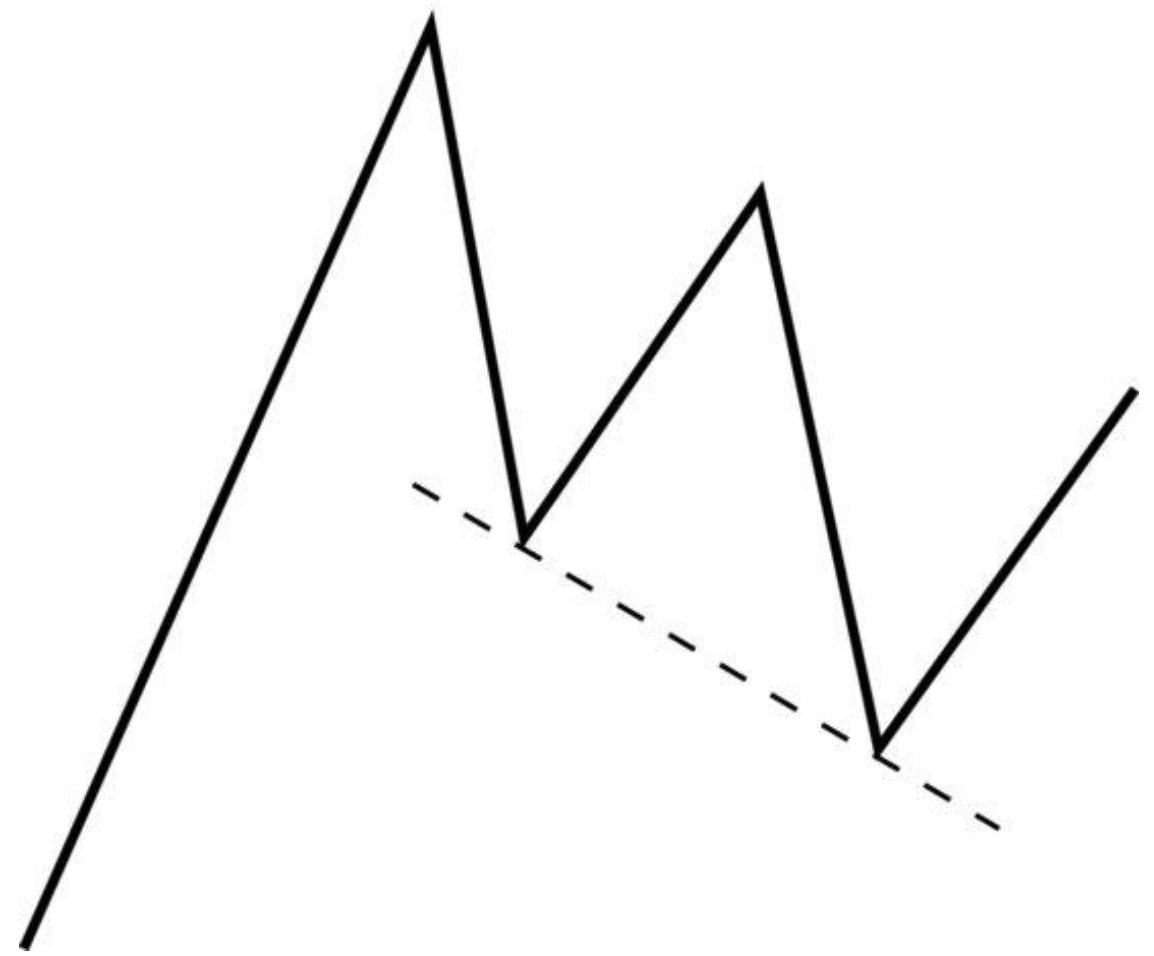
\includegraphics[width=0.4\linewidth]{pullback-slope-down}
\begin{itemize}
  \item Does not make sense to exit a trade that is within the loping level
\end{itemize}

\subsubsection{Trigger 1: Lower time frame climax}
\begin{enumerate}
  \item Draw a parallel trend line pullback
  \begin{enumerate}
    \item First draw a standard linear trendline for lower timeframe between higher lows in an uptrend (demand line) or lower highs for downtrend (supply line)
    \item Create a parallel line to the opposite side of the trend (attach to pivot highs in uptrend) BETWEEN the initial two anchor points for standard trend line. Also must not cut through prices between the two initial anchor points
  \end{enumerate}
  \item Price drops past support, but immediately recover within a few bars (lower time-frame climax), but should be clear from default timeframe
\end{enumerate}
Note this is not a buy-and-forget entry. Needs experience and to pay attention because most likely exhausiton below support happens in a single bar.

\subsubsection{Trigger 2: Bottom of support}
\begin{enumerate}
  \item See a bounce back in pullback. Draw horizontal line at peak.
  \item Buy when when price reaches support again.
  \item Must not be buying into 3rd or more test of support (ie, only buying after one bounce). If support is tested for third or more times, reduce exposure.
\end{enumerate}
\subsection{Stop}
\begin{itemize}
  \item Crucial to have a stop loss.
  \item Recommend to set one further away from pattern and add in a few cents beyond obvious levels
  \item Can change stops dramatically a few bars into a trade
  \item Can use a time stop
\end{itemize}
\subsection{Profit Target}
\begin{itemize}
  \item Most conservative profit target is previous pivot high of the setup leg
  \item Good exit plan allows taking partial profits and holding onto portion of position for further trend legs
  \item Can use MMO profit targets, but recommend to take majority or all profits even though trade has not quite reached the target
\end{itemize}
\subsection{Comments}







\end{document}
